\documentclass[final]{beamer}
\mode<presentation>{\usetheme{Lankton}}
\usepackage{amsmath,amsfonts,amssymb,pxfonts,xspace}
\usepackage{graphicx}
\usepackage[orientation=landscape,size=custom,width=121.92,height=91.44,scale=1,debug]{beamerposter} %width 48 inches, height 36 inches
%\usepackage[orientation=landscape,size=a0,scale=1.1,debug]{beamerposter}
% \usepackage{verbatim}
\usepackage{color}
% \definecolor{red}{RGB}{184,17,55}
\definecolor{red}{rgb}{0.8,0,0}
\def\red{\color{red}}

% \usepackage{graphicx}
% \usepackage{amsmath}
% \usepackage{dsfont}
% \usepackage{amssymb}
% % \usepackage{url}
% \usepackage{verbatim}
% \usepackage[mathlines]{lineno}
% \usepackage{color}

%%%%%%%%%%%%%%%%%%%%%%%%%%%%%%%%%%%%%%%

\newtheorem{dummy}{Lemma}
\newtheorem{vex}[dummy]{Example}
\newtheorem{thm}{Theorem}[section]
\newtheorem{claim}[thm]{Claim}
\newtheorem{quest}[thm]{Question}
\newtheorem{prop}[thm]{Proposition}
\newtheorem{cor}[thm]{Corollary}
\newtheorem{rem}[thm]{Remark}
\newtheorem{lem}[thm]{Lemma}
\newtheorem{ex}[thm]{Example}
\newtheorem{defn}[thm]{Definition}
\newtheorem{conj}[thm]{Conjecture}
\newtheorem{obs}[thm]{Observation}
\newtheorem{alg}[thm]{Algorithm}

% Shortcut Commands %
\newcommand{\rank}{\operatorname{rank}}
\newcommand{\mr}{\operatorname{mr}}
\newcommand{\mrp}{\operatorname{mr}_+}
\newcommand{\mrF}{\operatorname{mr}^F}
\newcommand{\mrFG}{\operatorname{mr}^F(G)}
\newcommand{\M}{\operatorname{M}}
\newcommand{\MF}{\operatorname{M}^F}
\newcommand{\Mp}{\operatorname{M}_+}
\newcommand{\Z}{\operatorname{Z}}
\newcommand{\Zo}{\operatorname{Z}_o}
\newcommand{\R}{\mathbb{R}}
%\newcommand{\Z}{\mathbb{Z}}
\newcommand{\CC}{\mathbb{C}}
\newcommand{\ZZ}{\mathbb{Z}_2}
\newcommand{\Nn}{\mathbb{N}}
\newcommand{\C}{\mathcal{C}}
\newcommand{\U}{\mathcal{U}}
\newcommand{\Q}{\mathcal{Q}}
\newcommand{\G}{\mathcal{G}}
\newcommand{\h}{\mathcal{H}}
\newcommand{\D}{\Gamma}
\newcommand{\p}{{P}}
\newcommand{\A}{\mathcal{A}}
\newcommand{\cyc}{\mathcal{C}}
\newcommand{\B}{\mathcal{B}}
\newcommand{\J}{\mathcal{J}}
\newcommand{\s}{\mathcal{S}}
\newcommand{\T}{\mathcal{T}}
\newcommand{\Rnn}{\R^{n\times n}}
\newcommand{\Rn}{\R^{n}}
\newcommand{\Cn}{\mathbb{C}^{n}}
\newcommand{\Cnn}{\mathbb{C}^{n\times n}}
\newcommand{\Znn}{\Z^{n\times n}}
\newcommand{\Zn}{\Z^{n}}
\newcommand{\range}{\operatorname{range}}
\newcommand{\re}{\operatorname{Re}}
\newcommand{\Gc}{\overline{G}}
\newcommand{\Gam}{\Gamma}
\newcommand{\bx}{{\bf x}}
\newcommand{\bv}{{\bf v}}
\newcommand{\bw}{{\bf w}}
\newcommand{\bu}{{\bf u}}
\newcommand{\by}{{\bf y}}
\newcommand{\bz}{{\bf z}}
\newcommand{\be}{{\bf e}}
\newcommand{\spec}{\sigma}
\newcommand{\nul}{\operatorname{null}}
\newcommand{\lcm}{\operatorname{lcm}}
\newcommand{\cond}{\operatorname{cond}}
\newcommand{\sgn}{\operatorname{sgn}}
\newcommand{\In}{\operatorname{In}}
\newcommand{\Out}{\operatorname{Out}}
\newcommand{\lam}{\lambda}
\newcommand{\lamc}{\overline \lambda}
\newcommand{\eps}{\varepsilon}
\newcommand{\tr}{\operatorname{tr}}
\newcommand{\n}{\{1,\dots,n\}}
\newcommand{\ones}{\ensuremath{\mathds{1}}} 
\newcommand{\Adp}{\A_{D^+}}
\newcommand{\ba}{\begin{array}}
\newcommand{\ea}{\end{array}}
\newcommand{\Ap}{{\A}^+}


%\numberwithin{theorem}{section}

\newcommand{\x}{\times}
\newcommand{\bit}{\begin{itemize}}
\newcommand{\eit}{\end{itemize}}
\newcommand{\ben}{\begin{enumerate}}
\newcommand{\een}{\end{enumerate}}
\newcommand{\bea}{\begin{eqnarray*}}
\newcommand{\eea}{\end{eqnarray*}}
\newcommand{\beq}{\begin{equation}}
\newcommand{\eeq}{\end{equation}}
\newcommand{\bpf}{\begin{proof}}
\newcommand{\epf}{\end{proof}}
\newcommand{\ms}{\medskip}
\newcommand{\noin}{\noindent}

\def\mtx#1{\begin{bmatrix} #1 \end{bmatrix}}
\newcommand{\ds}{\displaystyle}


%-- Header and footer information ----------------------------------
\newcommand{\footleft}{Joint work with: Joe Alameda, Emelie Curl, Armando Grez, Leslie Hogben, O'Neill Kingston,
\\Alex Schulte, and Michael Young}
\newcommand{\footright}{\small $^1$Department of Mathematics, Iowa State University, Ames, IA 50011 (ecurl@iastate.edu, ddyoung@iastate.edu)}
\title{(Derek Version) The Equivalence of the Maximum Nullity and the Zero Forcing Number of Generalized Petersen Graphs}
\author{Emelie Curl, Derek Young }
\institute{Iowa State University, Ames, IA}
%-------------------------------------------------------------------


%-- Main Document --------------------------------------------------
\begin{document}
\begin{frame}{}
\begin{columns}[t]


%-- Column 1 ---------------------------------------------------
\begin{column}{0.23\linewidth} 
o
\begin{block}{\red Background}
The maximum nullity of a simple graph $G$, denoted $\M(G)$, is defined to be the largest possible nullity over all symmetric real matrices whose $ij$th entry is nonzero exactly when $\{i,j\}$ is an edge in $G$ for $i\neq j$, and the {$ii$}th entry is any real number. The zero-forcing number of a simple graph $G$, denoted $\Z(G)$, is the minimum number of blue vertices needed to force all vertices of the graph blue by applying the color change rule. The motivation for this research is the longstanding question of characterizing graphs $G$ for which $\M(G) = \Z(G)$. Specifically, we focused on a family of graphs called the Generalized Petersen Graphs. We were able to identify two subfamilies of this larger family that have the desired property, however, to possibly expand our results to the entire family more effective tools with regards to maximum nullity will need to be developed.
\end{block}

\begin{block}{Definitions}     
\bit
      
% Positive Matrix% 
%\item A matrix $A\in\Rnn$ is \emph{\bf positive} if every entry of $A$ is positive. \newline
      
% EP matrix %
\item Let $V$ be a finite set. A {\color{blue}\emph{simple graph}} $G=(V,E)$ is a pair of sets, such that $E$ is a set of 2 element subsets of $V$. The elements of $V$ are called {\color{blue}\emph{vertices}} and the elements of $E$ are called {\color{blue}\emph{edges}}. 
\item Vertices $u$ and $v$ are {\color{blue}\emph{adjacent}} in $G$ if $uv \in E$. Let $v \in V$. A vertex $u$ is a {\color{blue}\emph{neighbor}} of $v$ if $uv \in E$. The {\color{blue}\emph{neighborhood}} of $v$, denoted by $N(v)$ is the set of neighbors of $v$.
\item For a graph $G$, the {\color{blue}\emph{adjacency matrix}} of $G$, denoted $A(G)$ is a matrix $A(G) = [a(G)_{ij}]$ such that $a(G)_{ij}$ is 1 if $ij \in E$, and $a(G)_{ij}$ is zero otherwise. 
\item For a graph $G$, the {\color{blue}\emph{set of symmetric matrices of $G$ over $\mathbb{R}$}}, denoted $\mathcal{S}(G)$,  is the set of matrices $A=[a_{ij}]$ such that $a_{ij}$ is non-zero if $ij\in E$, $a_{ij}$ is any number if $i=j$ and $a_{ij}$ is zero otherwise. 
\item The {\color{blue}\emph{minimum rank}} of $G$ is 
\[
\mr(G) := \min\{rank(A) \mid A \in \mathcal{S}(G)\}.
\]
\item The {\color{blue}\emph{maximum nullity}} of $G$ is defined as 
\[
M(G) = \max\{null(A) \mid A \in \mathcal{S}(G)\}.
\]
\item We define the {\color{blue}\emph{color change rule}} as follows: Suppose a graph $G$ has every vertex colored either blue or white, and $b$ is a blue vertex. If $b$ has exactly one white neighbor, $w$, then change the color of $w$ to blue. We say that $b$ {\color{blue}\emph{forces }}$w$.
\item Let $S \subseteq V$. The {\color{blue}\emph{final coloring of $S$}} is
	the result of initially coloring every vertex in $S$ blue and every
	vertex in $V \setminus S$ white, and then applying the color-change
	rule until no more color changes can be made. The set $S$ is called a
	{\color{blue}\emph{zero forcing set}} if the final coloring of $S$ is all blue. 
\item The {\color{blue}\emph{zero-forcing number}} of a graph $G$ is 
\[
Z(G) = \min\{|S| : S\text{ is a zero forcing set of }G\}.
\] 
%\item A \emph{ \bf sign pattern} % matrix} (or\emph{ sign pattern}) 
%is a matrix having entries in $\{+,-,0\}$. \newline

%\begin{center}{${\A}=\mtx{+ & - & + \\ 0 & - & + \\  + & + & 0 }$  is a $3\x3$ sign pattern.}\end{center}
             
        
%\ben
      
%\item $\B$ is a \emph{\bf subpattern} of $\A$.
%\item $\A$ is a \emph{\bf superpattern} of $\B$. \newline
     
% \een

    
% Positive Part %
%\item    
\eit
\end{block}

\begin{block}{Zero Forcing Example}
%\begin{center}
%%\includegraphics[scale=.12]{Traingle1PD.pdf}
\textbf{Claim:} The set $S = \{2,4\}$ is a zero forcing set and $\Z(G) = 2$.
\begin{figure}[h!]
\centering
\scalebox{1.30}{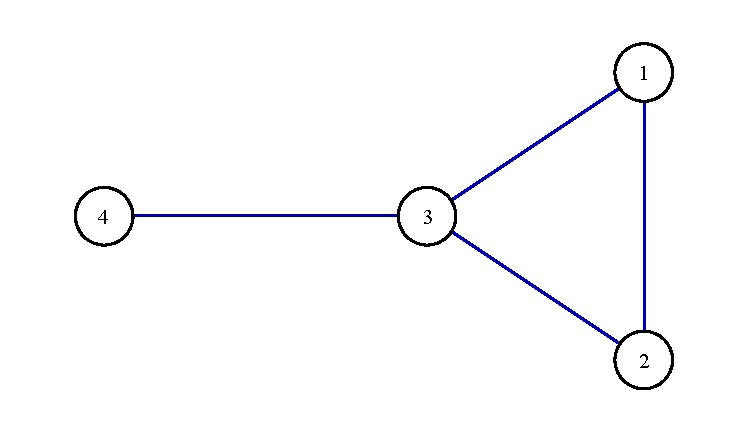
\includegraphics{Triangle1P.pdf}}
%\end{center}
\end{figure}

\end{block}

\end{column}%1

%-- Column 2 ---------------------------------------------------
\begin{column}{0.38\linewidth}
 

%-- Block 2-1
\begin{block}{Results Cited}
     
\bit

\item {\bf Theorem}[AIM Minimum Rank]
The zero forcing number provides an upper bound for the maximum nullity, $\M(G) \leq \Z(G)$, and therefore provides a lower bound on the minimum rank, $n-\Z(G) \leq \mr(G)$. 
\item {\bf Theorem}[AIM Minimum Rank]
$C_n \square P_2$ ($n-$Prism) for $n \geq 3, \quad\M(C_n \square P_2) = \Z(C_n \square P_2) = 4.$
\eit
\end{block}

\begin{block}{\red\Huge The Generalized Petersen Graphs}
A {\color{blue}\emph{Generalized Petersen Graph}} (GP), denoted $C_{n,k}$
is a graph such that 
$n \geq 3$ and $0 < k \leq \lfloor \frac{n-1}{2} \rfloor$
with vertex set and edge set
\[
V(C_{n,k}) = \{u_0, u_1, u_2, \ldots, u_{n-1}, v_0, v_1,
v_2, \ldots,
v_{n-1} \}
\] 
\[
E(C_{n,k}) = \{u_iu_{i+1},\, u_iv_i,\, v_jv_{j+k} \, |\, 0 \leq
i,j
\leq n-1\}
\] where subscripts are taken modulo $n$. [West]
\begin{figure}[h!] 
\centering
\scalebox{0.9}{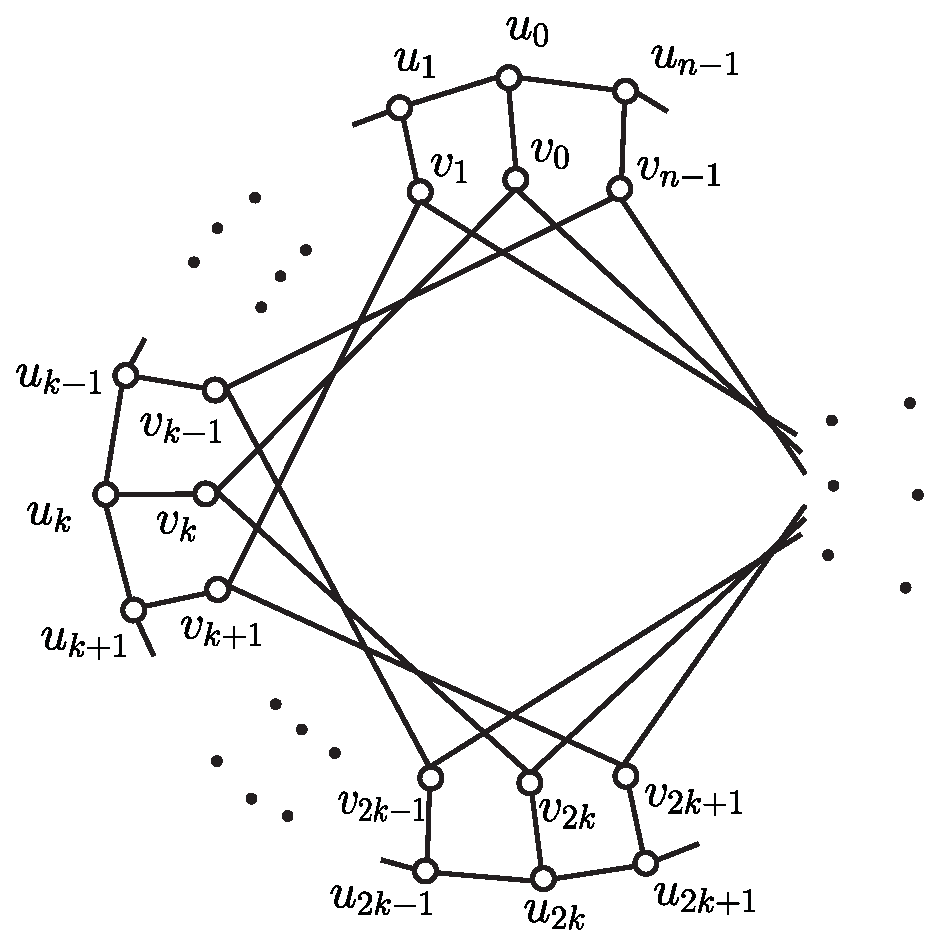
\includegraphics{genpetlabe.eps}}
\caption{Generalized Petersen Graph.}
\end{figure}


\end{block}

\begin{block}{The Adjacency Matrix of Generalized Petersen Graphs}
The following block matrix is the adjacency matrix for the Generealized
Petersen graph:
\[
\huge{A(C_{n,k}) = \begin{bmatrix} \huge{A(C_n)} & \huge{I_n}  \\
\huge{I_n}  & \huge{A(C_{n})'}    
\end{bmatrix}}
\]
where $I_n := n \times n $\text{ identity matrix}, $A(C_n) := $\text{ adjacency
matrix of the outer cycle on }n \text{ vertices,}\\ 
\text{and } $A(C_{n})' := $ \text{ adjacency matrix of the inner
cycle(s) and is a matrix with ones in the }$k$\text{th and }\\$n-k$\text{th super and sub diagonals and zeroes elsewhere.}
\end{block}

\begin{block}{Eigenvalue Property of Generalized Petersen Graphs} 
\bit
\item[]{\bf Lemma}
Suppose $\lambda$ is an eigenvalue of the adjacency matrix of $C_{n,k}$ with multiplicity $m$. Then, $\lambda$ is an eigenvalue of the adjacency matrix of $C_{nr,k}$ with multiplicity at least $m$ where $r \geq 1$.\\*[1cm]
\eit
\end{block}

\begin{block}{Sketch of Proof}
        
Suppose we have $\lambda$ and associated vector $\vec{x}=[x_0, \ldots, x_{n-1}, x_{n}, \ldots, x_{2n-1}]^T$
with adjacency matrix $A(C_{n,k}) = \begin{bmatrix} A(C_{n}) & I_{n}\\
I_{n} & A(C_n)' \end{bmatrix}.$\\
Then, $A(C_{n,k})\vec{x} = \lambda \vec{x}$ we get the equations (with $0 \leq j \leq n-1$):
$$x_{j-1} + x_{j+1} + x_{n+j} = \lambda x_j \text{ where }j-1,j,j+1 \text{ are taken }\bmod n$$
$$x_{j} + x_{n+k+j} + x_{2n-k+j} = \lambda x_j \text{ where }j \text{ is taken }\bmod n.$$
We show $A(C_{nr,k}) \vec{X_r} = \lambda \vec{X_r}$ for any $r \geq 1$ where:
$$A(C_{nr,k}) = \begin{bmatrix} A(C_{nr}) & I_{nr}\\
I_{nr} & A(C_{nr})' \end{bmatrix}$$
$$\vec{X_r} = [\underbrace{x_0, \ldots, x_{n-1}, \ldots, x_0, \ldots, x_{n-1}}_{r \text{ times }}, \underbrace{x_{n}, \ldots, x_{2n-1}, \ldots, x_{n}, \ldots, x_{2n-1}}_{r \text{ times }}]^T.$$
\end{block}


\end{column}%2
    
%-- Column 3 ---------------------------------------------------
\begin{column}{0.38 \linewidth}

\begin{block}{\red The Zero Forcing Number}
        {\bf Observation:} For any $ n \geq 3 $, $ \Z(C_{n,k}) \leq 2k + 2 $.
        
\textbf{Sketch of Proof:}
% \centering
\begin{itemize}
\item $S = \{v_0, u_0, \dots, u_{2k-1}, v_{2k-1}\}$ and apply the color change rule.\\
\item $S_0 = S \cup \{v_1, \dots, v_{2k-2}\}$ is the set of blue vertices
after the first force.\\
\textbf{Note:} If $S_0 $ is a zero forcing set then $S$ is a zero forcing set
and we are done.
\item Define $S_{j+1} = S_j \cup \{u_{2k+j},v_{2k+j}\}$ which implies
$S\subseteq S_0 \subseteq S_1 \subseteq \cdots \subseteq S_{n-2k}$. 
\item Since $S_{n-2k} = V(G)$ and $V(G)$ is a zero forcing set so is $S$.
\end{itemize}

\end{block}

\begin{block}{$C_{8,3}$ = M\"{o}bius - Kantor graph}
\textbf{Claim:} The M\"{o}bius-Kantor graph has a zero forcing set given in the previous proof.
\begin{figure}[h!]
\centering
\scalebox{.50}{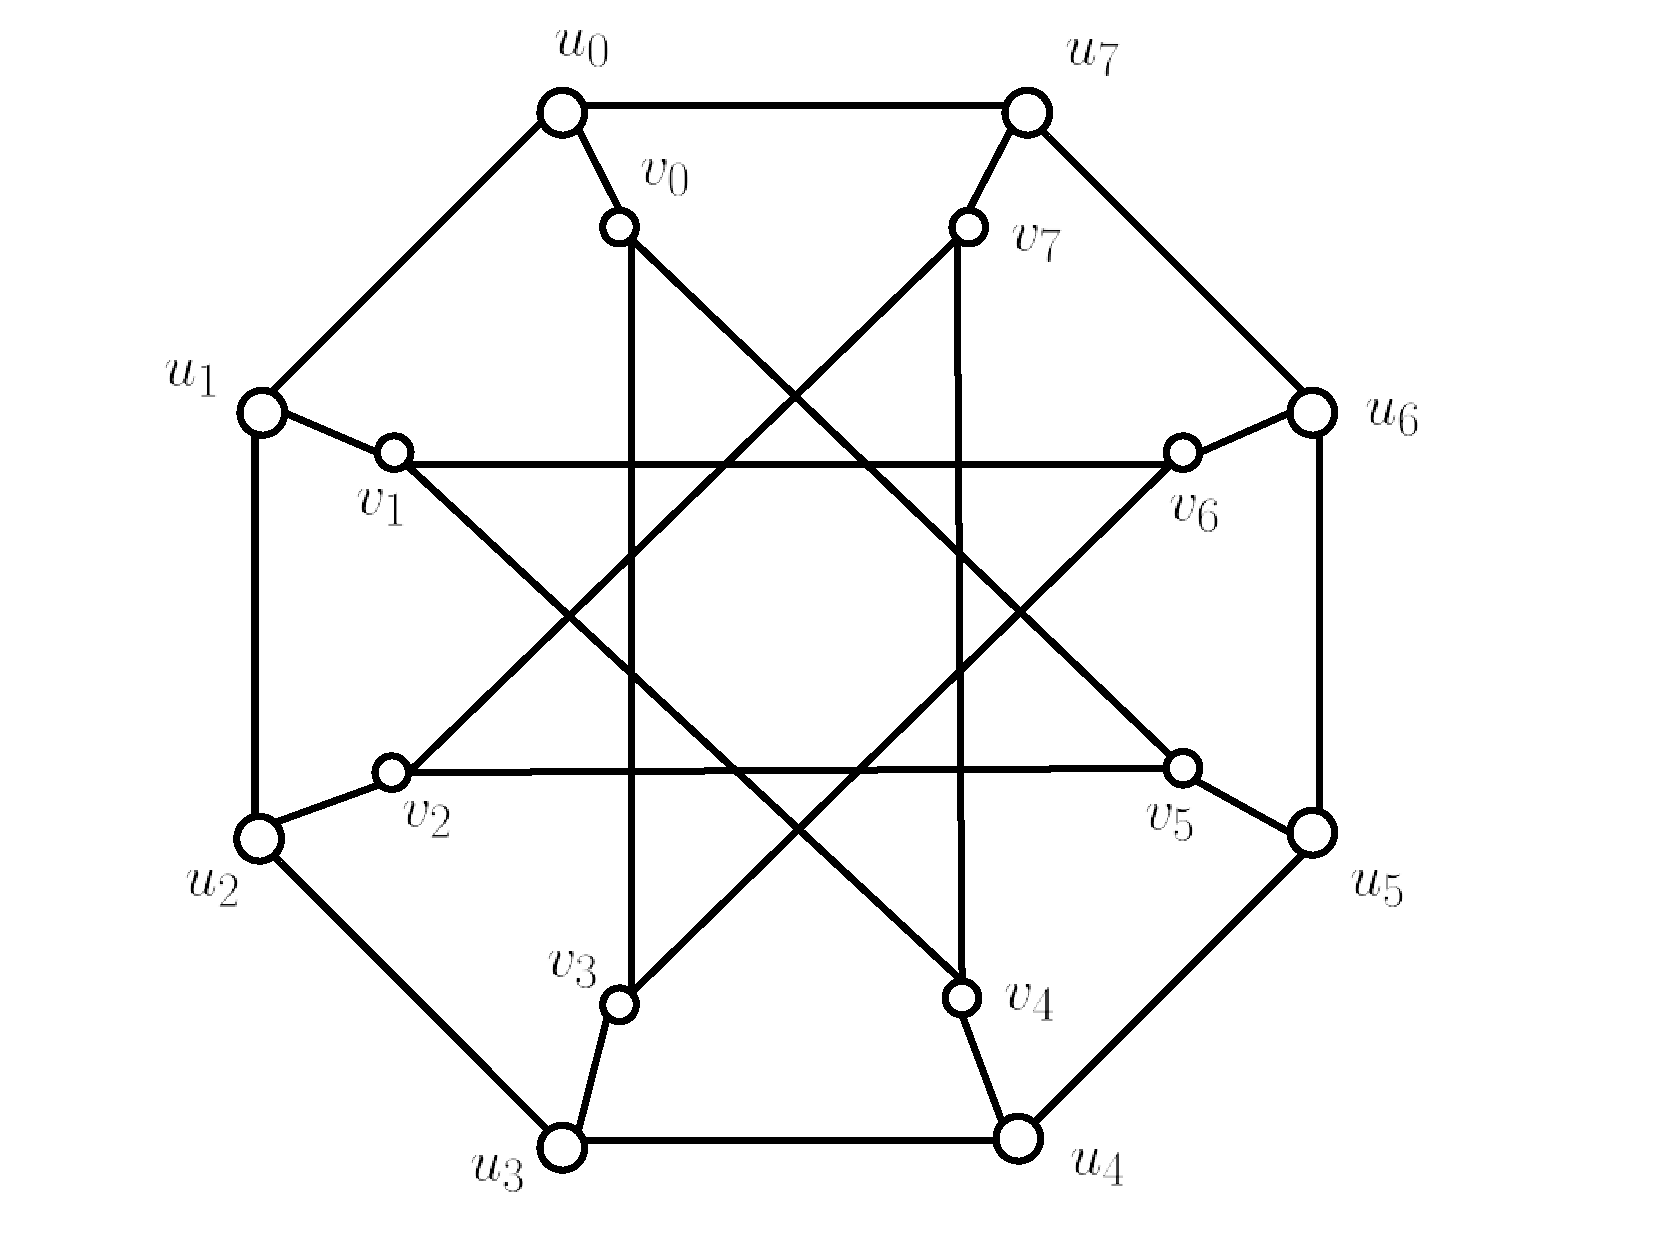
\includegraphics{gengraphsa.pdf}}
\end{figure}

\end{block}
        
\begin{block}{Main Results}
\bit
\item[]{\bf Theorem:} For any $n \geq 3$ and $0 <  k  \leq \frac{n-1}{2} $, such that there is $\lambda \in spec(A(C_{n,k}))$ such that the multiplicity of $\lambda$ is  $2k+2$, we have $\M(C_{n,k}) = \Z(C_{n,k}) = 2k+2$.

\item[]{\bf Corollary:} $\M(C_{15r,2}) = \Z(C_{15r,2}) = 6$ and 
$\M(C_{24r,5}) = \Z(C_{24r,5}) = 12$ for all $r \geq 1$.
\eit
\end{block}

\begin{block}{Sketch of Proof}
Immediately from the zero forcing observation (above), AIM Minimum Rank, and the eigenvalue property of GP graphs (left):
\[
2k+2 = \nul(A(C_{n,k}) - \lambda I) \leq \M(C_{n,k}) \leq \Z(C_{n,k}) \leq 2k+2.
\]
Then, use the above zero forcing observation and find an eigenvalue of the adjacency matrices of $C_{15,2}$ and $C_{24,5}$ respectively so that the multiplicity of  each eigenvalue is $2k+2$. These eigenvalues are $-2$ and $0$ respectively.
\end{block}

%\begin{block}{Other Results}
%\bit
%\item Define {\color{blue}\emph{bat graphs}} as follows: Let $B_0$ be the graph given by a $C_4$ with a leaf appended to each of two non-adjacent vertices. This graph has $\M(B_0) = \Z(B_0) = 2$ with its adjacency matrix being of minimum rank and a minimum zero forcing set being given by one leaf and one degree 2 vertex. Call the degree 3 vertices $x_1$ and $x_2$, the degree 2 vertices $y_1$ and $y_2$, and the leaves $y_3$ and $y_4$. This is called the basic bat graph, and any graph constructed by a sequence of twinning operations applied to $x_1$ or $x_2$ is a bat graph.
%\item {\bf Theorem:}  $\M(B) = \Z(B)$ for every bat graph $B$.
%\item Define a {\color{blue}\emph{jewel graph}} to be a $K_{r,r}$ where one edge is deleted. Define an \emph{$s,r$-jewel necklace}, $J_{s,r}$, to be a cycle of jewel graphs adjoined appropriately by edges between vertices with deg$(v) = r-1$. In this process no more than $1$ edge should cause such vertices to become adjacent to one another. Let $s$ be the number of copies of jewels in the cycle and $r$ represents the degree of the vertices. Note that this graph remains bipartite and $r$-regular. By definition we require that $r \geq 3$ and $s \geq 2$ (otherwise we would be examining a cycle ($r=2$), $s$ copies of $P_2$ ($r=1$), or a $K_{r,r}$ ($s=1$), for which maximum nullity and zero forcing are known).Note that $n = \mid J_{s,r}\mid = 2sr$.
%\item {\bf Theorem:} The double jewel necklace $J_{2,r}$ has $\mr(J_{2,r})=6$ and $\M(J_{2,r}) = \Z(J_{2,r})$ for $r \geq 3$.
%\eit
%\end{block}

\begin{block}{Future Work}
\bit
\item {\bf Conjecture:} Suppose $\lambda$ is an eigenvalue of $C_{s\cdot \ell, \lfloor \frac{(s \cdot \ell) - 1}{2} \rfloor }$ with multiplicity $m$, then $\lambda$ is an eigenvalue of $C_{s \cdot \ell^r, \lfloor \frac{(s \cdot \ell^r) - 1}{2} \rfloor}$ with multiplicity at least $m$, where $s \cdot \ell \geq 3$ and $r \geq 1$.
\item {\bf Conjecture:} Let $G =  C_{5\cdot 3^r, \lfloor \frac{1}{2}((5\cdot3^r)-1) \rfloor}$ where $r \geq 0$. Then $\M(G) = 6 = \Z(G)$. 
\item Find other subfamilies so that $\M = \Z$. 
\item Develop tools to find the maximum nullity of all GP graphs.
\eit
\end{block}

\begin{block}{Commonly Known Generalized Petersen Graphs}
\bit
\item $C_{n,1}$ -  $C_n \square P_2$ ($n-$Prism) for $n \geq 3$, $\quad\M(C_{n,1}) = \Z(C_{n,1}) = 4$ [AIM Minimum Rank]
\item $C_{5,2}$ - The Petersen graph,  $\hspace{1.9cm} \M(C_{5,2}) = \Z(C_{5,2}) = 5$ [AIM Minimum Rank]
\item $C_{6,2}$ - The  D\"{u}rer  graph 
\item $C_{8,3}$ - The M\"{o}bius - Kantor graph 
\item $C_{10,2}$ - The Dodecahedron graph 
\item $C_{10,3}$ - The Desargues graph  
\item $C_{12,5}$ - The Nauru graph
\eit
\end{block}
        
\begin{block}{References}
\begin{thebibliography}{20}
      
\bibitem{AIM08} AIM Minimum Rank -- Special Graphs Work Group (F. Barioli, W. Barrett, S. Butler, S. M. Cioab\u{a}, D. Cvetkovi\'c, S. M. Fallat, C. Godsil, W. Haemers, L. Hogben,  R. Mikkelson,  S. Narayan,  O. Pryporova,   I. Sciriha,  W. So,   D. Stevanovi\'c,  H. van der Holst, K. Vander Meulen,  A. Wangsness).  Zero forcing sets and the minimum rank  of graphs.   {\em Linear Algebra App.}, 428 (2008),  1628--1648.
\bibitem{WestGraphTheory} West, Douglas Brent. Introduction to graph theory. Vol. 2. Upper Saddle River: Prentice hall, 2001.
\end{thebibliography}
\end{block}

\end{column}%3

\end{columns}

\end{frame}

\end{document} 
